% ============================================================================
% Capítulo 9 — Gerenciamento ágil do projeto
% ============================================================================
\section{GERENCIAMENTO ÁGIL DO PROJETO}

\subsection{Organização do trabalho}

O projeto foi organizado em duas frentes paralelas, com escopos e diretórios
disjuntos: a Parte A, responsável pelo núcleo corporativo, pela aplicação Web,
pela API, pelo banco de dados e pela infraestrutura; e a Parte B, responsável
pelo aplicativo mobile. Cada frente trabalhou em uma cópia isolada do repositório
(\emph{worktree}) e em uma branch própria, integrada à linha principal ao final
de cada ciclo.

A separação reduziu conflitos e permitiu que o contrato OpenAPI funcionasse
como interface de coordenação: a Parte B desenvolveu contra um servidor simulado
e trocou para o serviço real sem alteração de telas.

\subsection{Product Backlog}

O Product Backlog foi estruturado em épicos e histórias, priorizados por valor
para a cooperativa e por dependência técnica. A Tabela~\ref{tab:backlog} apresenta
os principais itens, com estimativa em pontos de história e prioridade.

\begin{table}[H]
  \centering
  \caption{Product Backlog resumido}
  \label{tab:backlog}
  \fontsize{9}{11}\selectfont
  \begin{tabular}{L{1.2cm}L{6.6cm}L{1.6cm}L{2.0cm}L{2.0cm}}
    \toprule
    \textbf{ID} & \textbf{História de usuário} & \textbf{Pontos} & \textbf{Prioridade} & \textbf{Sprint} \\
    \midrule
    US01 & Como administrador, quero cadastrar e aprovar produtores & 5 & Alta & 1 \\
    US02 & Como administrador, quero manter o catálogo de produtos & 3 & Alta & 1 \\
    US03 & Como produtor, quero registrar a colheita em lote & 8 & Alta & 1 \\
    US04 & Como comprador, quero criar pedidos com itens e lote & 8 & Alta & 2 \\
    US05 & Como administrador, quero programar rotas e gerar entregas & 5 & Média & 2 \\
    US06 & Como motorista, quero atualizar o status da entrega & 5 & Alta & 2 \\
    US07 & Como motorista, quero enviar foto e GPS como evidência & 8 & Alta & 3 \\
    US08 & Como produtor, quero registrar lote sem conexão & 13 & Alta & 3 \\
    US09 & Como administrador, quero emitir faturas a partir de pedidos & 5 & Média & 3 \\
    US10 & Como gestor, quero ver indicadores e relatórios & 5 & Média & 3 \\
    US11 & Como usuário, quero acessibilidade e política de privacidade & 3 & Média & 4 \\
    US12 & Como equipe, quero pipeline de integração e entrega & 5 & Média & 4 \\
    \bottomrule
  \end{tabular}

  \vspace{2pt}
  {\fontsize{9}{11}\selectfont\itshape Fonte: elaborado pelo autor (2026)}
\end{table}

\subsection{Sprints}

O cronograma foi dividido em quatro sprints de duas semanas, descritas na
Tabela~\ref{tab:sprints}. Cada sprint terminou com incremento demonstrável,
compilação sem avisos e testes aprovados.

\begin{table}[H]
  \centering
  \caption{Sprint Backlog}
  \label{tab:sprints}
  \fontsize{9.5}{11.5}\selectfont
  \begin{tabular}{L{1.4cm}L{6.6cm}L{6.4cm}}
    \toprule
    \textbf{Sprint} & \textbf{Objetivo} & \textbf{Entrega} \\
    \midrule
    1 & Fundação: domínio, banco, autenticação e catálogo & Migrations,
      script do banco, login Web e API, cadastros básicos \\
    2 & Fluxo comercial: pedidos, rotas e entregas & Pedido com itens, rota
      com entregas, atualização de status \\
    3 & Evidência, faturamento e offline & Foto com GPS, fatura idempotente,
      fila offline e sincronização \\
    4 & Qualidade, acessibilidade, DevOps e integração & Relatórios,
      auditoria, pipeline, APK e validação ponta a ponta \\
    \bottomrule
  \end{tabular}

  \vspace{2pt}
  {\fontsize{10}{12}\selectfont\itshape Fonte: elaborado pelo autor (2026)}
\end{table}

\subsection{Quadro Kanban}

O fluxo de trabalho foi visualizado em um quadro Kanban com cinco colunas:
Backlog, A Fazer, Em Progresso, Em Revisão e Concluído. A Figura~\ref{fig:kanban}
representa o quadro ao final da terceira sprint, com a distribuição típica de
itens.

\begin{figure}[H]
  \centering
  \caption{Quadro Kanban ao final da terceira sprint}
  \label{fig:kanban}
  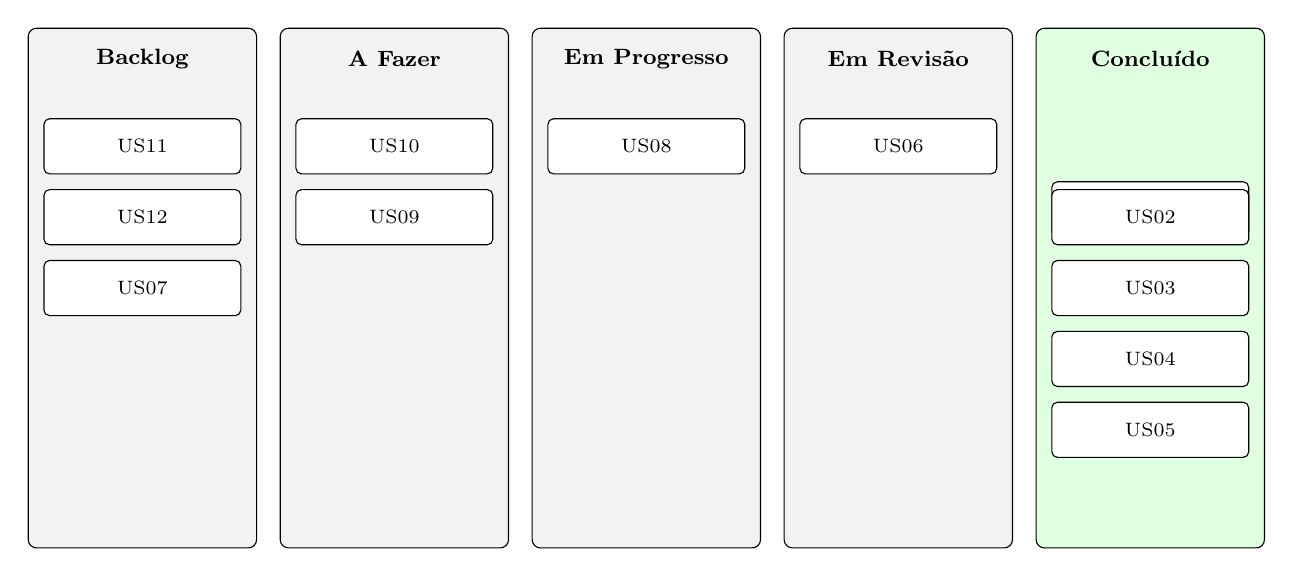
\begin{tikzpicture}[
    col/.style={draw, rounded corners=3pt, minimum width=29mm, minimum height=66mm,
      align=center, font=\fontsize{8}{9}\selectfont},
    cartao/.style={draw, fill=white, rounded corners=2pt, minimum width=25mm,
      minimum height=7mm, align=center, font=\fontsize{7}{8.5}\selectfont, inner sep=1pt}
  ]
    \node[col, fill=gray!10] (c1) at (0,0) {};
    \node[col, fill=gray!10] (c2) at (3.2,0) {};
    \node[col, fill=gray!10] (c3) at (6.4,0) {};
    \node[col, fill=gray!10] (c4) at (9.6,0) {};
    \node[col, fill=green!12] (c5) at (12.8,0) {};

    \node[font=\fontsize{8}{9}\selectfont\bfseries] at (c1.north) [yshift=-4mm] {Backlog};
    \node[font=\fontsize{8}{9}\selectfont\bfseries] at (c2.north) [yshift=-4mm] {A Fazer};
    \node[font=\fontsize{8}{9}\selectfont\bfseries] at (c3.north) [yshift=-4mm] {Em Progresso};
    \node[font=\fontsize{8}{9}\selectfont\bfseries] at (c4.north) [yshift=-4mm] {Em Revisão};
    \node[font=\fontsize{8}{9}\selectfont\bfseries] at (c5.north) [yshift=-4mm] {Concluído};

    \node[cartao] at ([yshift=18mm]c1.center) {US11};
    \node[cartao] at ([yshift=9mm]c1.center) {US12};
    \node[cartao] at ([yshift=0mm]c1.center) {US07};
    \node[cartao] at ([yshift=18mm]c2.center) {US10};
    \node[cartao] at ([yshift=9mm]c2.center) {US09};
    \node[cartao] at ([yshift=18mm]c3.center) {US08};
    \node[cartao] at ([yshift=18mm]c4.center) {US06};
    \node[cartao] at ([yshift=10mm]c5.center) {US01};
    \node[cartao] at ([yshift=9mm]c5.center) {US02};
    \node[cartao] at ([yshift=0mm]c5.center) {US03};
    \node[cartao] at ([yshift=-9mm]c5.center) {US04};
    \node[cartao] at ([yshift=-18mm]c5.center) {US05};
  \end{tikzpicture}
  \fonte{elaborado pelo autor (2026)}
\end{figure}

\subsection{Definition of Ready e Definition of Done}

Uma história era considerada \emph{pronta} (Definition of Ready) quando
apresentava critério de aceite verificável, protótipo ou descrição de interface,
dependências identificadas e estimativa acordada. Era considerada
\emph{concluída} (Definition of Done) quando o código compilava sem avisos, os
testes passavam, as validações de entrada estavam implementadas, a interface
respeitava os critérios de acessibilidade, a documentação era atualizada e o
commit era feito em português com mensagem descritiva.

\subsection{Riscos e lições aprendidas}

Os principais riscos do projeto foram a indisponibilidade de infraestrutura para
validação, a divergência entre contrato e implementação e a baixa familiaridade
do usuário final com tecnologia. As mitigações adotadas foram, respectivamente:
validação do banco com contêiner e execução da aplicação contra dados reais;
geração automática dos tipos do mobile a partir do contrato; e desenho de telas
simples, com operação offline e linguagem direta.

Como lição aprendida, destaca-se o valor de entregas pequenas e verificáveis: a
divisão em incrementos permitiu identificar cedo falhas de integração, como o
envio de evidência em certos aparelhos Android, e corrigi-las sem comprometer o
cronograma.
